\documentclass[]{report}
\usepackage{graphicx, float,}
\usepackage{hyperref}
\usepackage[export]{adjustbox}

\title{\centering CSP334 : Computer Networks \\Lab Assignment No 4\\Assignment on HTTP}
\author{\LARGE Sahil\\2016UCS0008}

% to use proper section numbering in the report type 
\renewcommand{\thesection}{\arabic{section}}

\begin{document} 

\maketitle

%%%%%%%%%%%%%%%%%%%%%%%%%%%%%%%%%%%%%%%%%%%%%%%%
\section{The Basic HTTP GET/ Response Interaction:}
File: \textit{simple1.html}
\subsection{HTTP Version of browser and server:}
\begin{figure}[H]
	\vspace{0pt}
	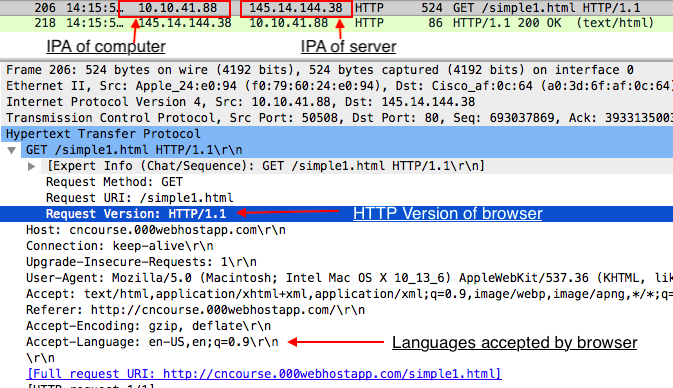
\includegraphics[height = 200pt, keepaspectratio]{Snapshots/q1/simple1/1_1.png}
\end{figure}
As highlighted, version \textbf{1.1} is used by both browser and server. 
\subsection{Languages accepted by the browser:}
As shown above, \textbf{English} language is accepted. 
\subsection{IPA of computer and \textit{cncourse} web server:}
IPA of computer is $10.10.41.88$ and that of server is $145.14.144.38$. 
\subsection{Status code returned from server to the browser: \textit{200}}
\begin{figure}[H]
	\vspace{0pt}
	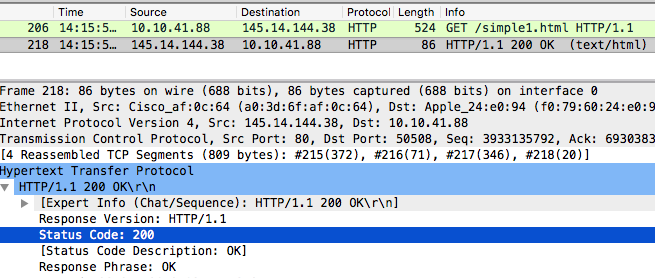
\includegraphics[height = 100pt, keepaspectratio]{Snapshots/q1/simple1/1_4.png}
\end{figure}
\subsection{HTML file last modified at the server:}
There is no \textit{last-modified} header in the HTTP packet. 
\subsection{Bytes of content returned to the browser:}
\begin{figure}[H]
  	\vspace{0pt}
  	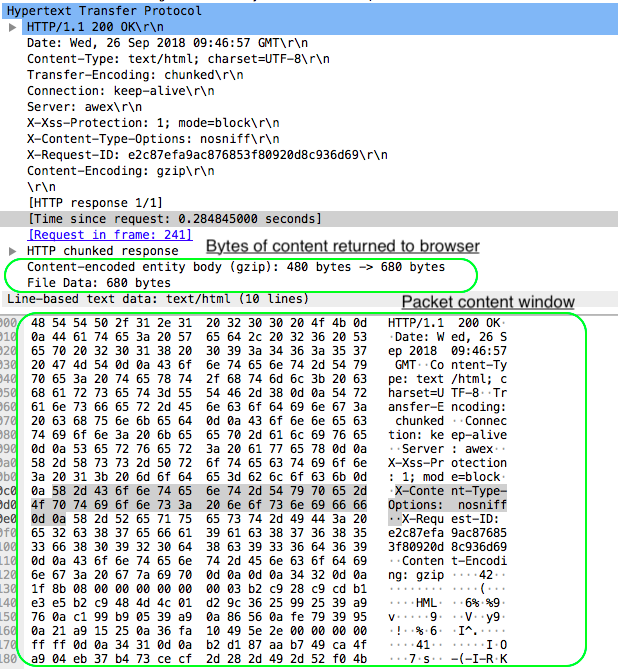
\includegraphics[height = 300pt, keepaspectratio]{Snapshots/q1/simple1/1_7.png}
\end{figure}
As highlighted, 480 bytes are returned to browser in \textit{gzip} format which is then uncompressed to 680 bytes by the browser.
\subsection{Headers not displayed in the packet-listing window:}
As seen in the packet content window, all the headers shown in the packet-listing window are only displayed, so there is NO additional header present.
\subsection{No. of request sent by browser and responded by server:}
\begin{figure}[H]
	\vspace{0pt}
	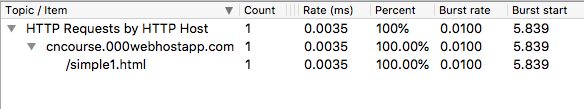
\includegraphics[height = 75pt, keepaspectratio]{Snapshots/q1/simple1/1_8.png}
\end{figure}
There is one request sent by the browser to the \textit{simple1.html} file on the server, and same is responded back by the server. 
\subsection{HTTP traffic flow graph showing the packet exchanges between the client and the server:}
The \textit{HTTP traffic flow} graph is obtained from the \textbf{Statistics - Flow Graph} option and then checking the option \textit{Limit to display filter} as the filter chosen is HTTP.
\begin{figure}[H]
	\vspace{0pt}
	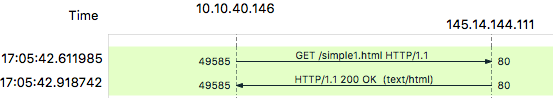
\includegraphics[height = 75pt, keepaspectratio]{Snapshots/q1/simple1/1_9.png}
\end{figure}
\subsection{File \textit{simple2.html}:}
\textbf{Last modified} information is not available for the \textit{html} file but for the \textit{GIF} image loaded along with this html, it is displayed below.
\begin{figure}[H]
	\vspace{0pt}
	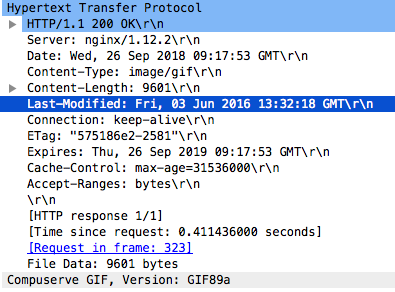
\includegraphics[height = 150pt, keepaspectratio]{Snapshots/q1/simple2/1_2_5.png}
\end{figure}
\textbf{Bytes of content} returned for the HTML file is $572$ bytes. That for the GIF is 9601 bytes.
\begin{figure}[H]
	\vspace{0pt}
	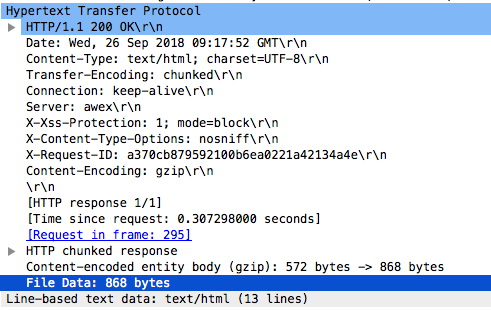
\includegraphics[height = 150pt, keepaspectratio]{Snapshots/q1/simple2/1_2_6.png}
\end{figure}
\textbf{No. of requests sent by the browser and responded by the server} are both $2$, as shown below. 
\begin{figure}[H]
	\vspace{0pt}
	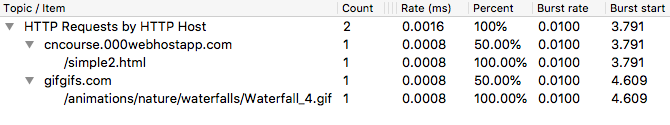
\includegraphics[height = 70pt, keepaspectratio]{Snapshots/q1/simple2/1_2_8.png}
\end{figure}
\textbf{HTTP Traffic Flow graph:}
\begin{figure}[H]
	\vspace{0pt}
	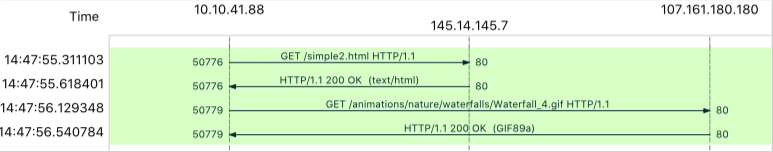
\includegraphics[height = 80pt, keepaspectratio]{Snapshots/q1/simple2/1_2_9.png}
\end{figure}
\subsection{File \textit{simple3.html}:}
\textbf{Last modified} information is not available for the \textit{simple3.html} file.
\begin{figure}[H]
	\vspace{0pt}
	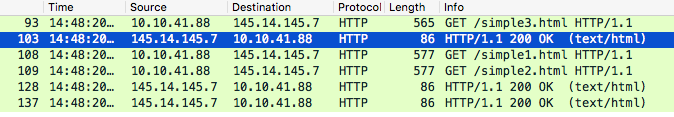
\includegraphics[height = 70pt, keepaspectratio]{Snapshots/q1/simple3/1_III.png}
\end{figure}
\textbf{Bytes of content} returned for the HTML file is $138$ bytes for \textit{simple3.html}. It also loads \textit{simple1.html} and \textit{simple2.html} whose sizes were mentioned earlier. 
\begin{figure}[H]
	\vspace{0pt}
	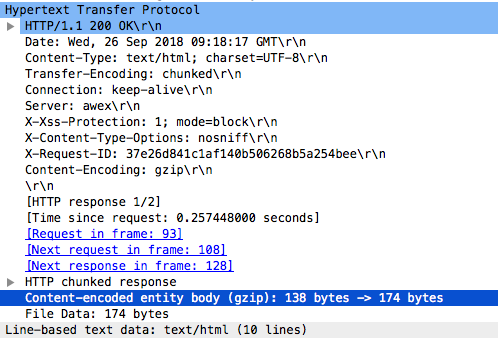
\includegraphics[height = 150pt, keepaspectratio]{Snapshots/q1/simple3/1_3_6.png}
\end{figure}
\textbf{No. of requests sent by the browser and responded by the server} are both $3$, as shown below. 
\begin{figure}[H]
	\vspace{0pt}
	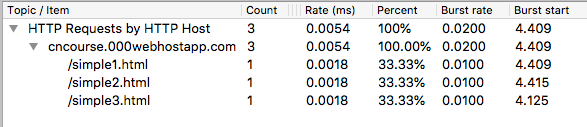
\includegraphics[height = 70pt, keepaspectratio]{Snapshots/q1/simple3/1_3_8.png}
\end{figure}
\textbf{HTTP Traffic Flow graph:}
\begin{figure}[H]
	\vspace{0pt}
	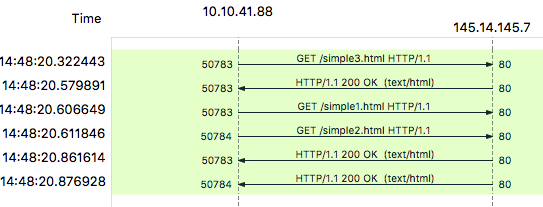
\includegraphics[height = 130pt, keepaspectratio]{Snapshots/q1/simple3/1_3_9.png}
\end{figure}
\subsection{File \textit{simple4.html}:}
\begin{figure}[H]
	\vspace{0pt}
	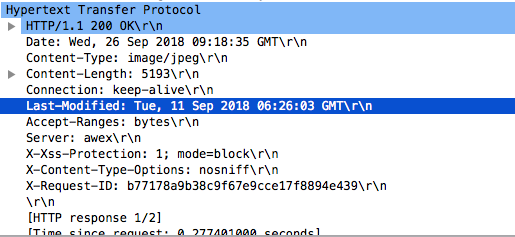
\includegraphics[height = 110pt, keepaspectratio]{Snapshots/q1/simple4/1_4_5.png}
\end{figure}
\textbf{Last modified} information is not available for the \textit{simple4.html} file but its present for the JPEG image files loaded from another server, as shown above for one such image. \\ 
\textbf{Bytes of content} returned for the HTML file is $535$ bytes for \textit{simple4.html}. It also loads 10 other image files.
\begin{figure}[H]
	\vspace{0pt}
	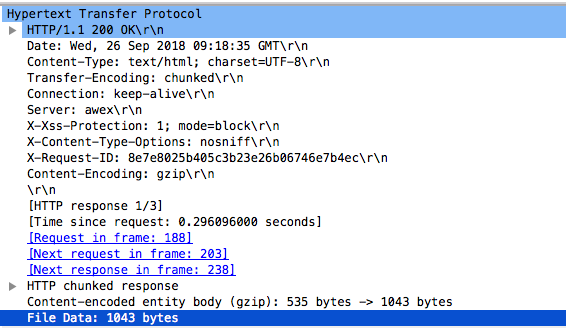
\includegraphics[height = 160pt, keepaspectratio]{Snapshots/q1/simple4/1_4_6.png}
\end{figure}
\textbf{No. of requests sent by the browser and responded by the server} are both $11$, as shown below. \\
\begin{figure}[H]
	\vspace{0pt}
	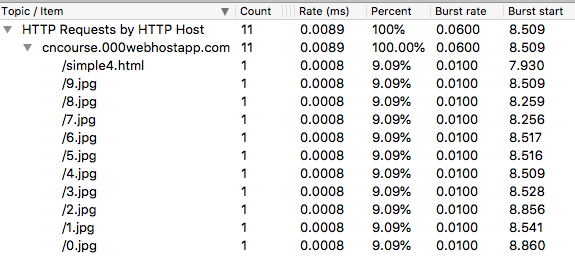
\includegraphics[height = 150pt, keepaspectratio]{Snapshots/q1/simple4/1_4_8.png}
\end{figure}
\textbf{HTTP Traffic Flow graph:}
\begin{figure}[H]
	\vspace{0pt}
	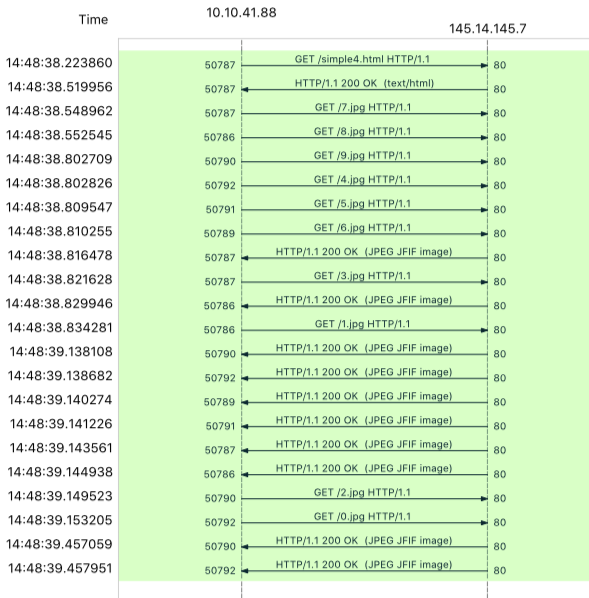
\includegraphics[height = 300pt, keepaspectratio]{Snapshots/q1/simple4/1_4_9.png}
\end{figure}
\subsubsection{Whether images downloaded serially or parallely:}
The image downloads occurred \textit{parallelly}. We can say so since in the above traffic flow graph, its clearly visible that the requests for the images 7.jpg, 8.jpg, 9.jpg, ..., all were made in a single go without waiting for response of either of the image to be available. The first response is available after 6 images were already requested. \\ \\
\subsection{Time required to access the pdf file:}
\begin{figure}[H]
	\vspace{0pt}
	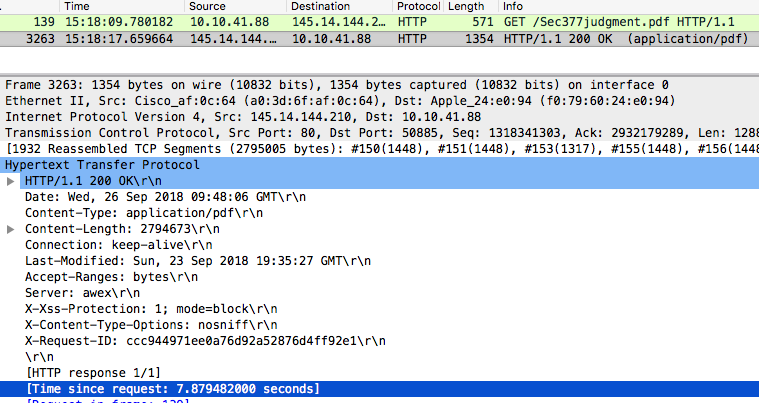
\includegraphics[height = 170pt, keepaspectratio]{Snapshots/q1/1_13.png}
\end{figure}
The time required as highlighted = $7.88$ seconds. \\ \\ \\ \\
\subsection{Table for time required to access each of the files:}
\large
\begin{center}
	\begin{tabular}{ |p{1cm}|p{3cm}|p{8cm}|  }
		\hline
		S.No & File Name & Time Required to access the file (in seconds)	\\
		\hline
		1. & simple1.html & $0.284$ \\
		\hline
		2. & simple2.html & $0.307$ \\
		\hline
		3. & simple3.html & $0.257$\\
		\hline
		4. & PDF file & $7.88$ \\
		\hline
		5. & Large Text file & $1.167$\\
		\hline
	\end{tabular} 
\end{center}
%%%%%%%%%%%%%%%%%%%%%%%%%%%%%%%%%%%%%%%%%%%%%%%%


\section{The HTTP CONDITIONAL GET/Response Interaction:}
The 4 requests were captured as shown below:
\begin{figure}[H]
	\vspace{0pt}
	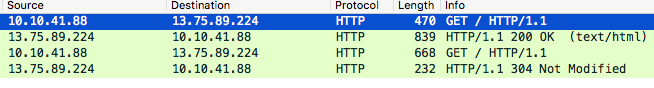
\includegraphics[height = 50pt, keepaspectratio]{Snapshots/q2/2.png}
\end{figure}
\subsection{First HTTP GET request from the browser to the server:}
\begin{figure}[H]
	\vspace{0pt}
	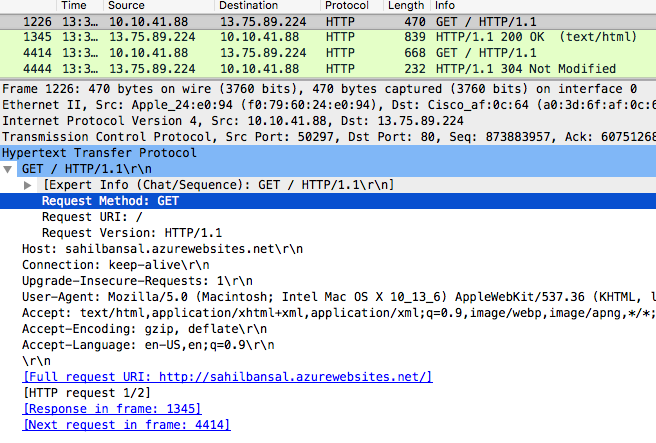
\includegraphics[height = 250pt, keepaspectratio]{Snapshots/q2/2_1.png}
\end{figure}
There is no \textbf{IF-MODIFIED-SINCE} header in this GET request.
\subsection{Contents of the server response:}
\begin{figure}[H]
	\vspace{0pt}
	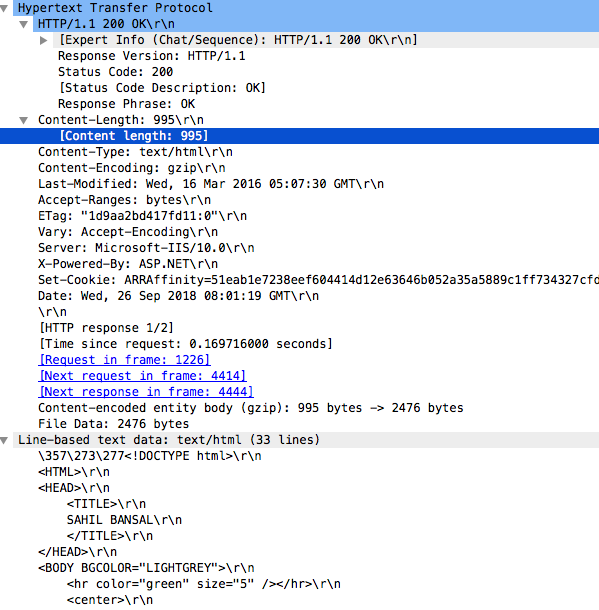
\includegraphics[height = 250pt, keepaspectratio]{Snapshots/q2/2_2.png}
\end{figure}
Yes, the server has explicitly responded with the content of the file since the \textit{content length} has a positive value and also the HTML file is visible as shown.
\subsection{Second HTTP GET request from the browser to the server: }
\begin{figure}[H]
	\vspace{0pt}
	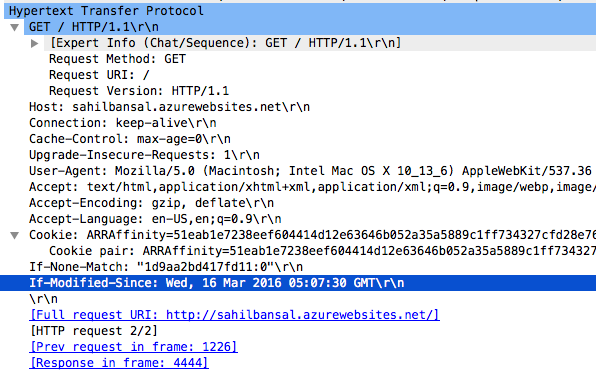
\includegraphics[height = 200pt, keepaspectratio]{Snapshots/q2/2_3.png}
\end{figure}
Yes, now we can see an \textbf{IF-MODIFIED-SINCE} header in the HTTP GET request. The value of the header is the date when the file was last modified on the server side. It shows \textit{Wed, Mar 16, 2016} as the last modified date.
\subsection{HTTP status code and phrase returned from the server in response to 2nd HTTP GET:}
\begin{figure}[H]
	\vspace{0pt}
	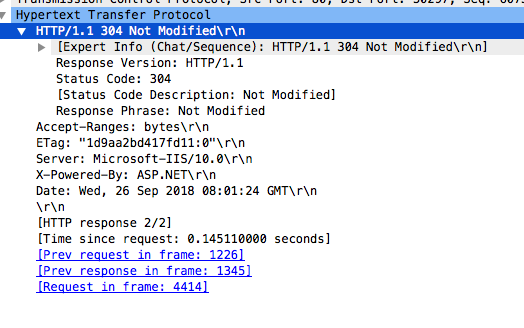
\includegraphics[height = 170pt, keepaspectratio]{Snapshots/q2/2_4.png}
\end{figure}
The status code is \textbf{304} and the response phrase is \textbf{Not Modified} in response to the 2nd HTTP GET request. The server did not explicitly return the content of the file this time since there is no content length header visible, as well as no content visible after two cr-lf present after the Date Header. \\
This happens because the client sent an IF-MODIFIED GET request, in which the server responds with the content only when the file has been modified on the server after the date of previous entry of the file in the cache accessbile by client. Otherwise, it just sends a 304-Not Modified response. 
%%%%%%%%%%%%%%%%%%%%%%%%%%%%%%%%%%%%%%%%%%%%%%%%


\section{Retrieving Long Documents:}
\subsection{HTTP GET request messages sent by the browser:}
\begin{figure}[H]
	\vspace{0pt}
	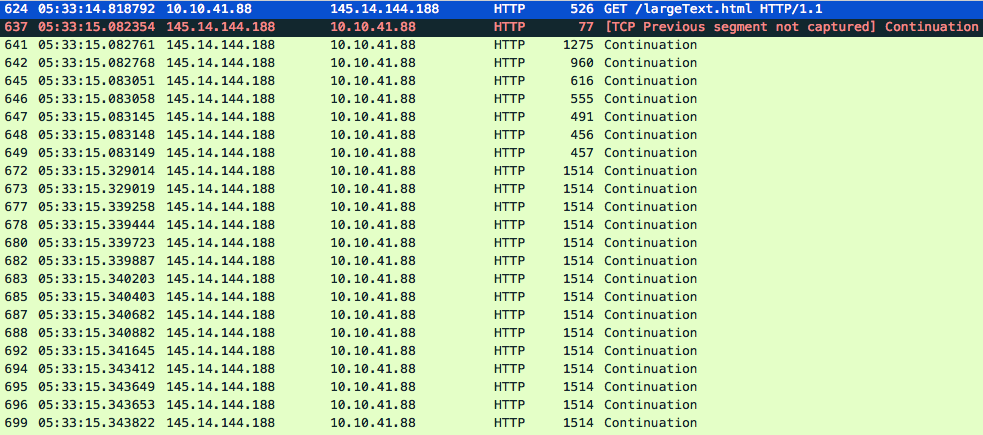
\includegraphics[height = 200pt, keepaspectratio]{Snapshots/q3/3_1.png}
\end{figure}
\begin{figure}[H]
	\vspace{0pt}
	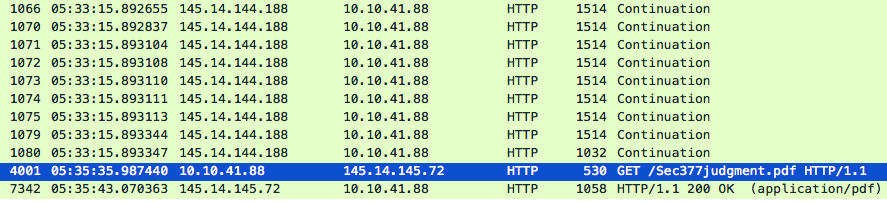
\includegraphics[height = 100pt, keepaspectratio]{Snapshots/q3/3_2.png}
\end{figure}
The browser sent 2 HTTP GET requests, one for the pdf file and other for the large text file since both requests were made in the same wireshark session. Both the requests are highlighted above. The packet numbers $624$ and $4001$ in the trace contain the HTTP GET message. 
\subsection{Packet no in trace containing the status code and phrase associated with the response to the HTTP GET request:}
We receive \textit{TCP Continuation} message for the large text file requested, as shown by packet no. $637$ highlighted in black above. A \textbf{200 OK} response is received for the pdf file requested as shown below. The response is the packet no. $4001$ in the above trace.
\begin{figure}[H]
	\vspace{0pt}
	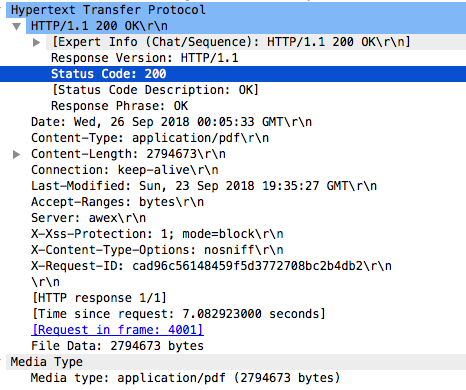
\includegraphics[height = 170pt, keepaspectratio]{Snapshots/q3/3_3.png}
\end{figure}
\subsection{Status code and phrase in the response:}
The status code is \textbf{200} and the response phrase is \textbf{OK}.
\subsection{No. of data-containing TCP segments needed to carry the single HTTP response and the text of the file:}
\begin{figure}[H]
	\vspace{0pt}
	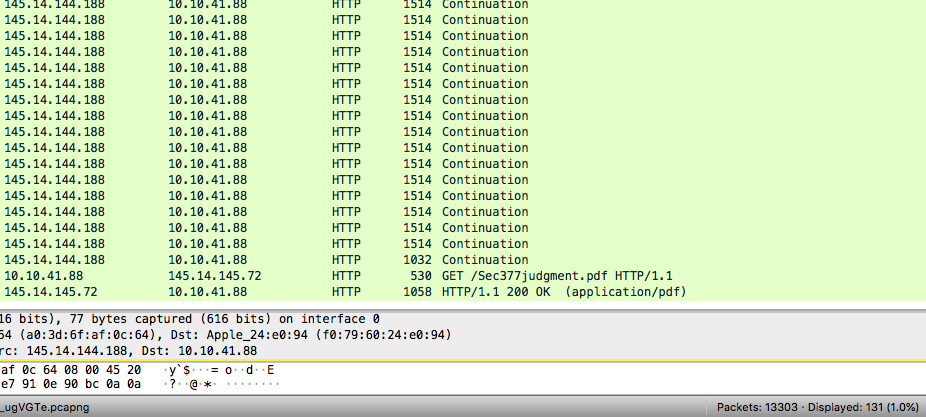
\includegraphics[height = 170pt, keepaspectratio]{Snapshots/q3/3_4.png}
\end{figure}
In total, there are $131$ HTTP packets were displayed, as shown in bottom right corner here, out of which 2 packets are for the pdf file, whereas in the remaining $129$ packets, $1$ is for the GET request and $1$ is for the HTTP response, so, in total $127$ data containing TCP segments were needed to carry the text of the file. 
%%%%%%%%%%%%%%%%%%%%%%%%%%%%%%%%%%%%%%%%%%%%%%%%


\section{HTML Documents with CGI Script:}
\begin{figure}[H]
	\vspace{0pt}
	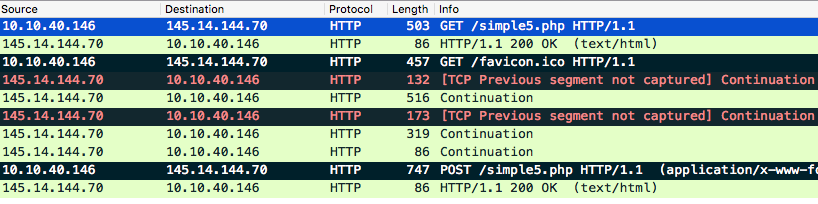
\includegraphics[height = 100pt, keepaspectratio]{Snapshots/q4/4.png}
\end{figure}
\subsection{Method used in the HTTP message:}
GET method is used to get the simple5.php file whereas POST method is also used to send the input taken from user to the server.
\subsection{No. of HTTP request messages sent by the browser:}
Total 3 HTTP request messages are sent by the browser.
\subsection{IPA to which the requests are sent:}
The IPA to which the requests are sent is $145.14.144.70$.
%%%%%%%%%%%%%%%%%%%%%%%%%%%%%%%%%%%%%%%%%%%%%%%%


\section{HTTP Authentication:}
\begin{figure}[H]
	\vspace{0pt}
	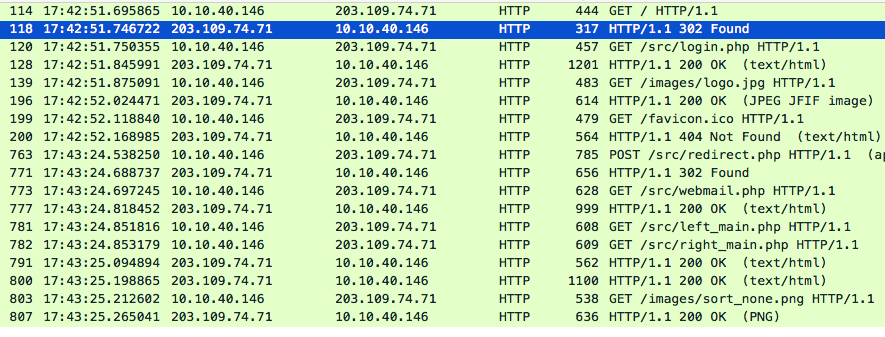
\includegraphics[height = 150pt, keepaspectratio]{Snapshots/q5/5_1.png}
\end{figure}
\subsection{Server response to the initial HTTP GET message:}
\begin{figure}[H]
	\vspace{0pt}
	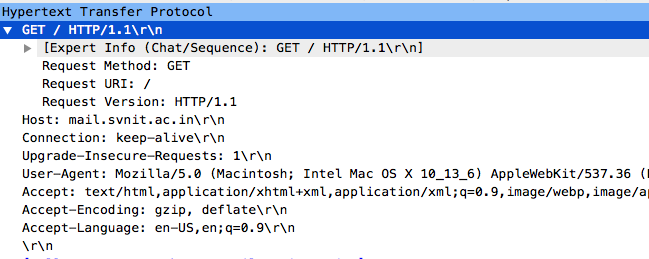
\includegraphics[height = 150pt, keepaspectratio]{Snapshots/q5/5_1_1.png}
\end{figure}
The status code is $302$ and the response phrase is \textbf{Found}, in response to the initial GET message which is shown above.
\subsection{New field included in HTTP GET message when browser sends request for 2nd time:}
\begin{figure}[H]
	\vspace{0pt}
	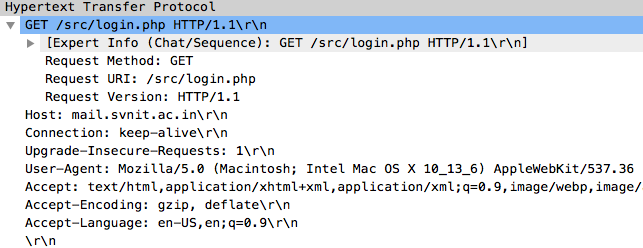
\includegraphics[height = 150pt, keepaspectratio]{Snapshots/q5/5_2.png}
\end{figure}
Considering the 2nd GET request sent by browser and comparing the HTTP message with previous one, we find that no new filed is included. 
\subsection{Content of packet in wireshark where password is displayed:}
\begin{figure}[H]
	\vspace{0pt}
	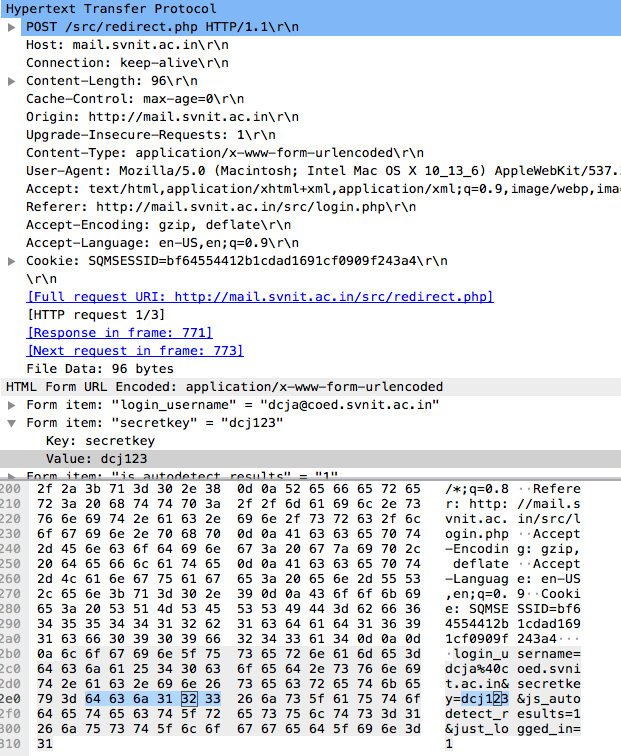
\includegraphics[height = 300pt, keepaspectratio]{Snapshots/q5/5_3.png}
\end{figure}
The password is highlighted in the packet content window with light blue color. 
%%%%%%%%%%%%%%%%%%%%%%%%%%%%%%%%%%%%%%%%%%%%%%%%

\end{document}